\section{Espectro de radiofrecuencias}
De la página del Ente Nacional de Comunicaciones (ENACOM): "El Espectro Radioeléctrico es el conjunto de frecuencias que, conforme a la tecnología disponible, pueden ser empleadas para emitir ondas que permitan transportar información. La manera en cómo está atribuido el Espectro Radioeléctrico en nuestro país se puede consultar en el "Cuadro de Atribución de Bandas de Frecuencias de la República Argentina", al que abreviadamente se lo conoce como CABFRA."

El espectro es considerado un recurso natural, de carácter limitado,  sobre el cual el estado tiene soberanía. Por lo tanto, se lo divide en bandas atribuidas a distintos servicios y sistemas de comunicaciones. A continuación se presenta una figura con las atribuciones según el CABFRA. 

Considerando esta tabla, se buscó sintonizar una frecuencia que no perteneciera a una emisora de radio o TV. El resultado se puede observar en (\ref{fig:hola}) Se sintonizó la frecuencia 301.5 MHz, que corresponde a alguna de las tres aplicaciones de la Figura (\ref{fig:noradionitelev}). A pesar de que pudieron observarse picos de potencia en el analizador, al conectar los parlantes sólo se escucharon pitidos intermitentes. Esto puede deberse a que la señal sintonizada era digital y el analizador es incapaz de interpretarla.

\begin{figure}[H]
	\centering
	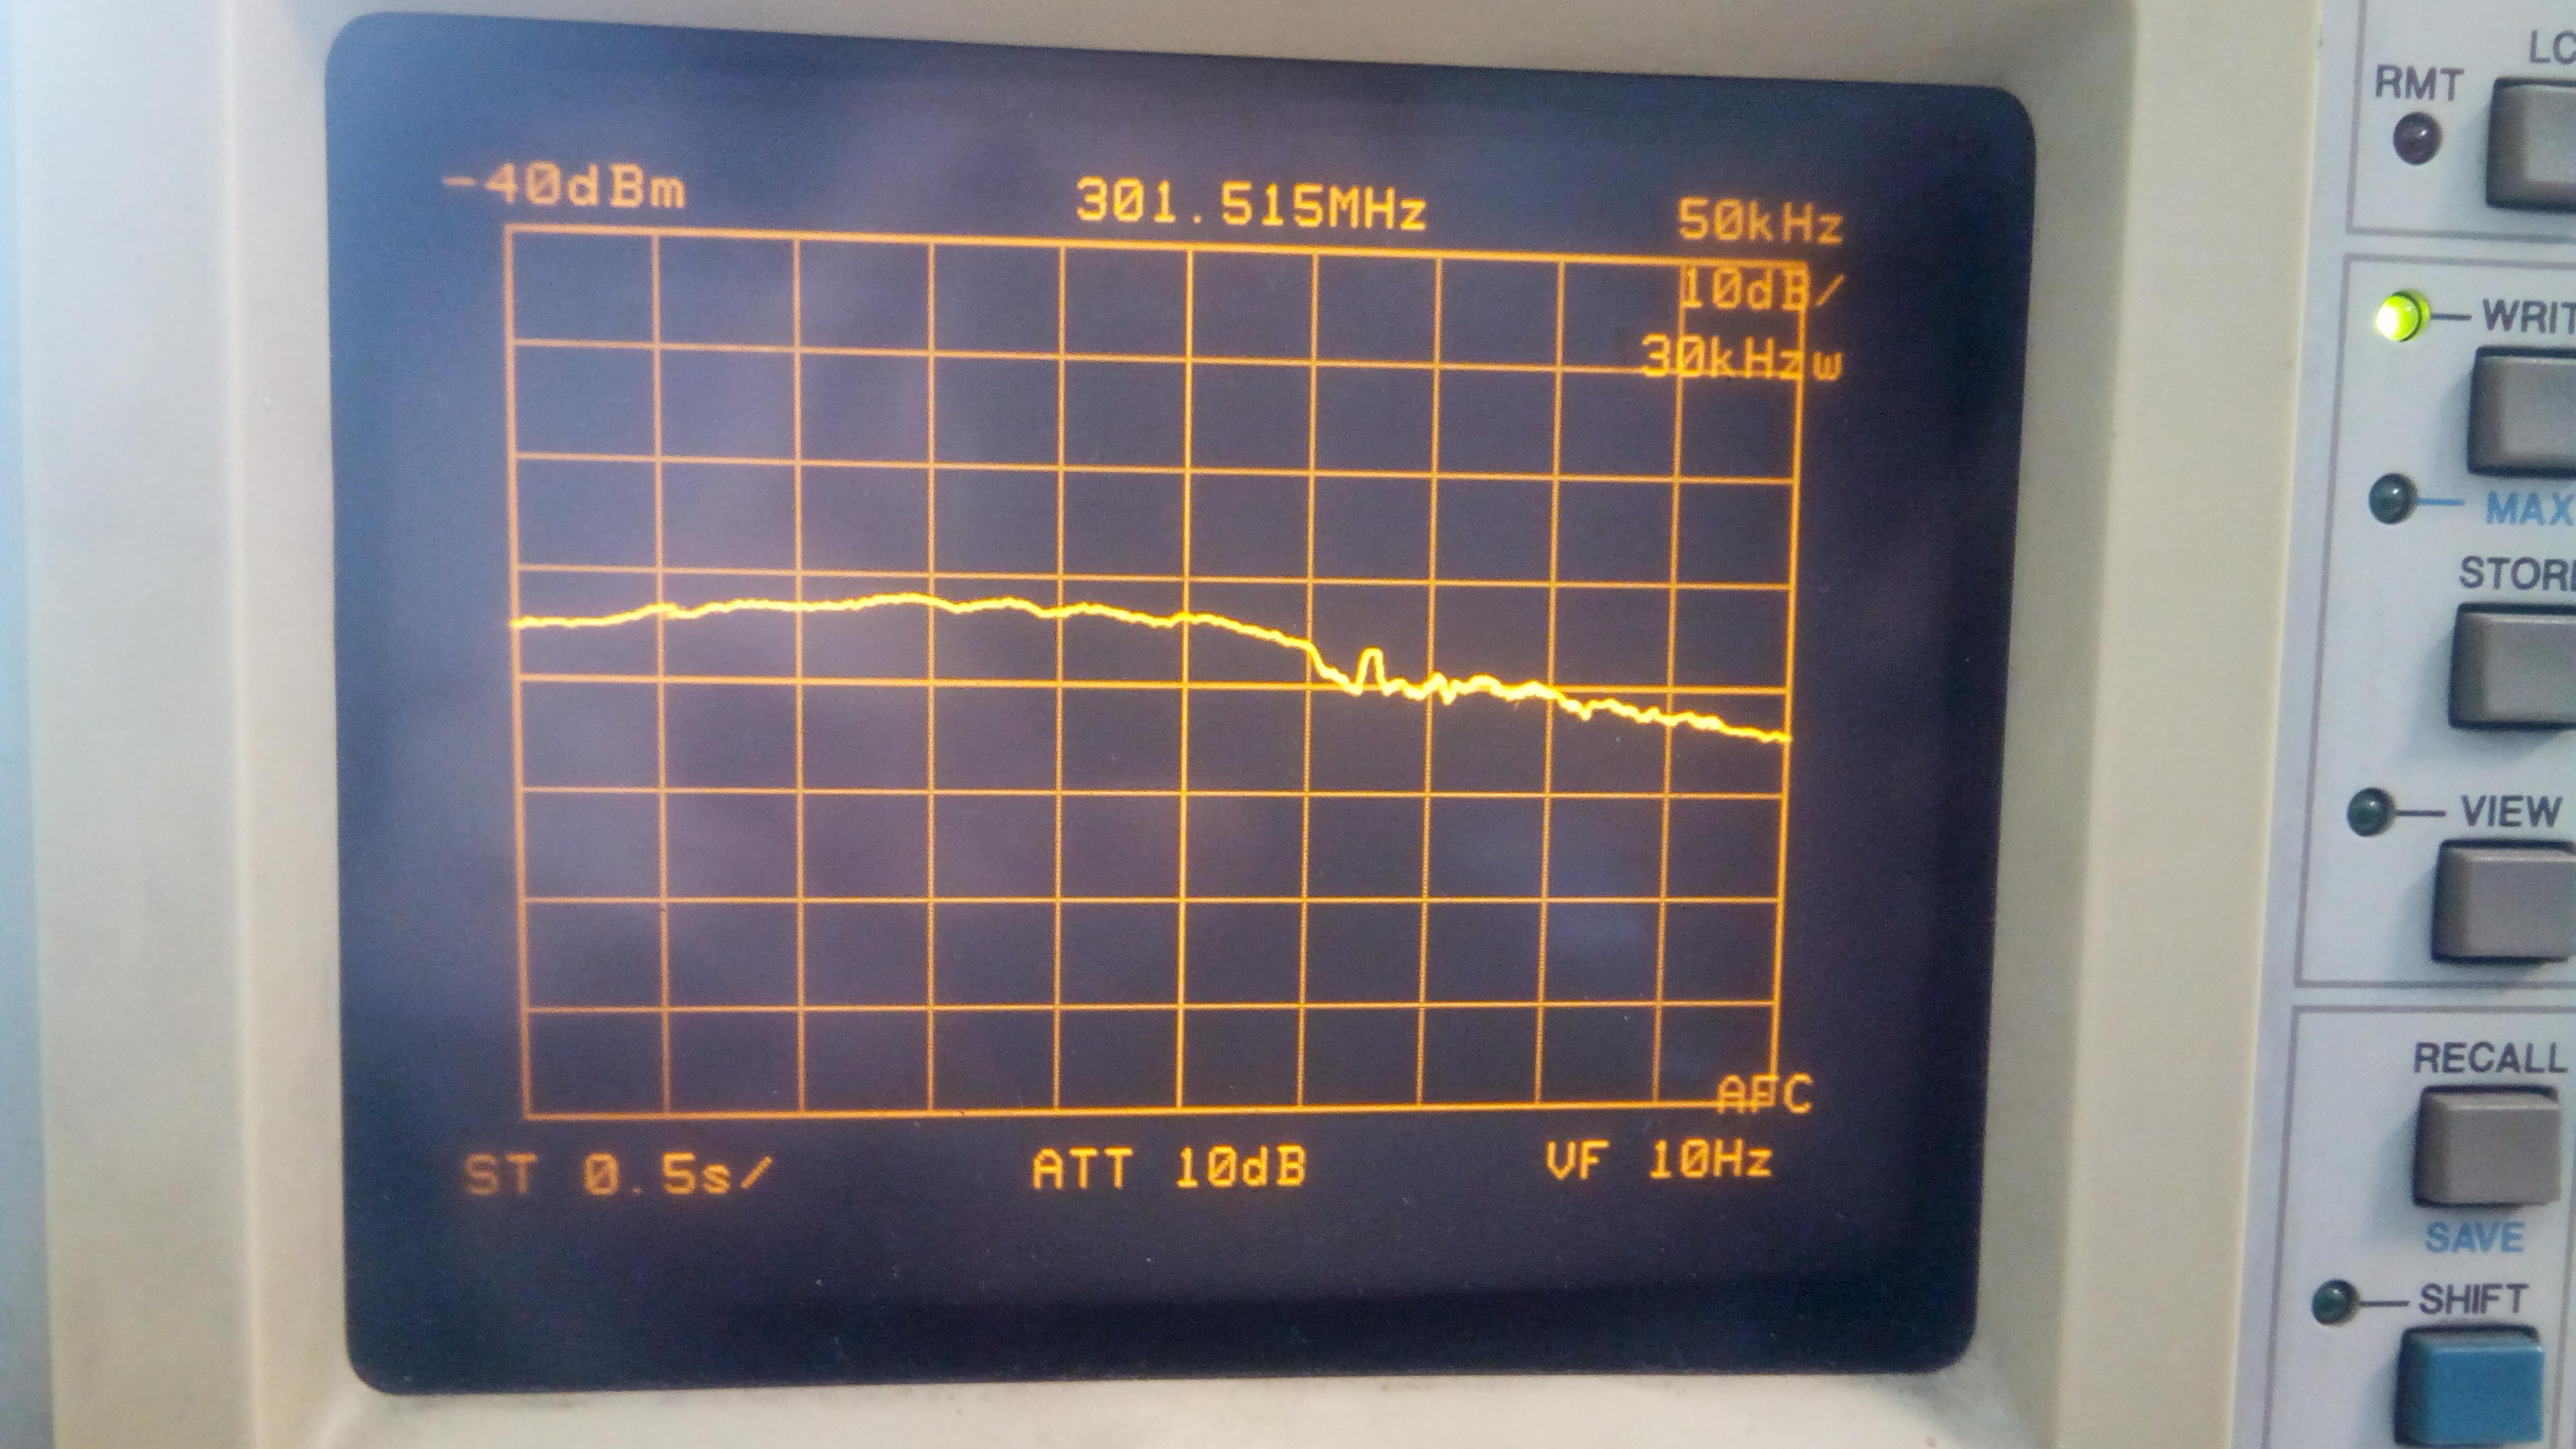
\includegraphics[width=0.9\textwidth]{/ImagenesEjercicio5-6y7/notvnoradio301MHz.jpg}
\caption{Espectro de la frecuencia analizada}
	\label{fig:hola}
\end{figure}

\begin{figure}[H]
	\centering
	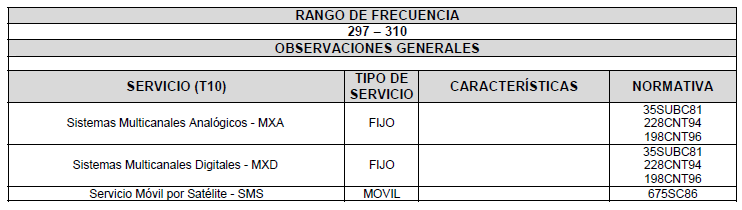
\includegraphics[width=0.9\textwidth]{/ImagenesEjercicio5-6y7/norh.png}
\caption{Aplicaciones en el rango de frecuencias analizado}
	\label{fig:noradionitelev}
\end{figure}

\begin{figure}[H]
	\centering
	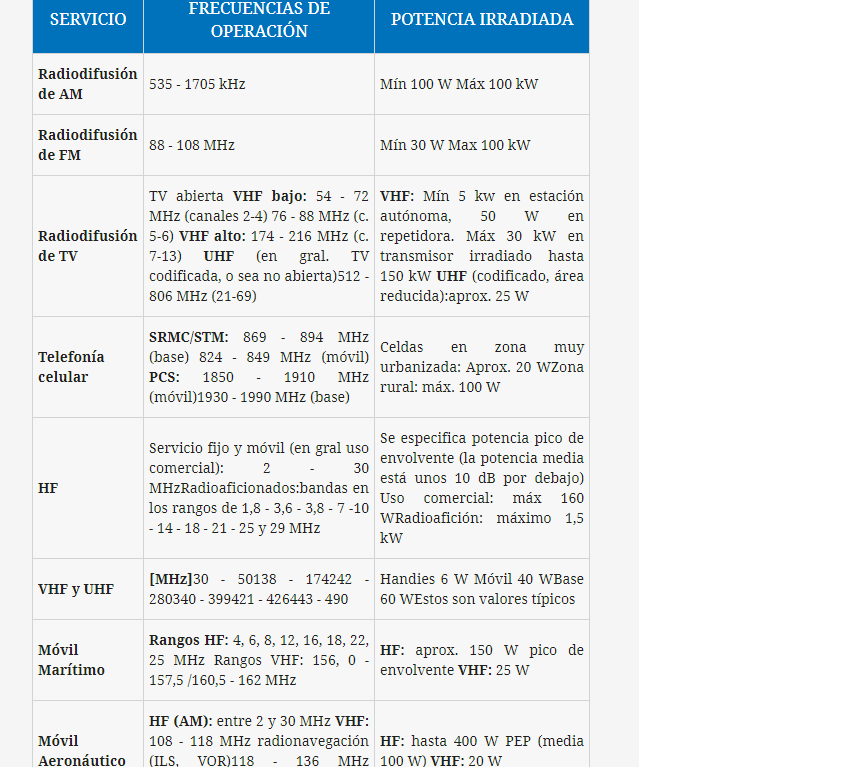
\includegraphics[width=0.97\textwidth]{/ImagenesEjercicio5-6y7/espectr.png}
	\caption{Atribución de bandas de frecuencia}
	\label{fig:esqcond}
\end{figure}

\section{Banda FM}

El espectro FM está dividido en siete categorías (de la A a la G) según el radio de servicio. A continuación se presenta una tabla tomada de la página web oficial del ENACOM en la que se muestra la división de bandas por categorías.

\begin{table}[H]
\centering
\begin{tabular}{|c|c|}
\hline
CATEGORÍA & \begin{tabular}[c]{@{}l@{}}RADIO DE ÁREA ESTIMADA\\ (48 dB$\mu$ V/m - 250 $\mu$V/m)\\ Km.\end{tabular} \\ \hline
A         & 90                                                                                            \\ \hline
B         & 80                                                                                            \\ \hline
C         & 70                                                                                            \\ \hline
D         & 45                                                                                            \\ \hline
E         & 28                                                                                            \\ \hline
F         & 22                                                                                            \\ \hline
G         & 9,5                                                                                           \\ \hline
\end{tabular}
\end{table}

Dentro de estas categorías yacen $100$ canales de $200 KHz$ cada uno. Estos van desde el canal $201$ con frecuencia $88,1 MHz$, hasta el canal 300 con frecuencia $107,9 MHz$.

Se buscó sintonizar alguna estación de radio y escucharla con unos parlantes conectados al analizador de espectros. Primero se sintonizó la estación Mega 98.3, con frecuencia 98.3 MHz, correspondiente al canal 277. En la figura \ref{fig:mega} puede observarse una imagen del espectro de la estación. La potencia de la portadora es de aproximadamente $-42 dBm$. Luego se sintonizó la emisora Aspen, con frecuencia 102.3 MHz, correspondiente al canal 297. En la figura \ref{fig:aspen} se observa el espectro medido para la estación. La potencia de la portadora se midió en aproximadamente $-35 dBm$. En ambos casos se logró un sonido con poca interferencia.

\begin{figure}[H]
	\centering
	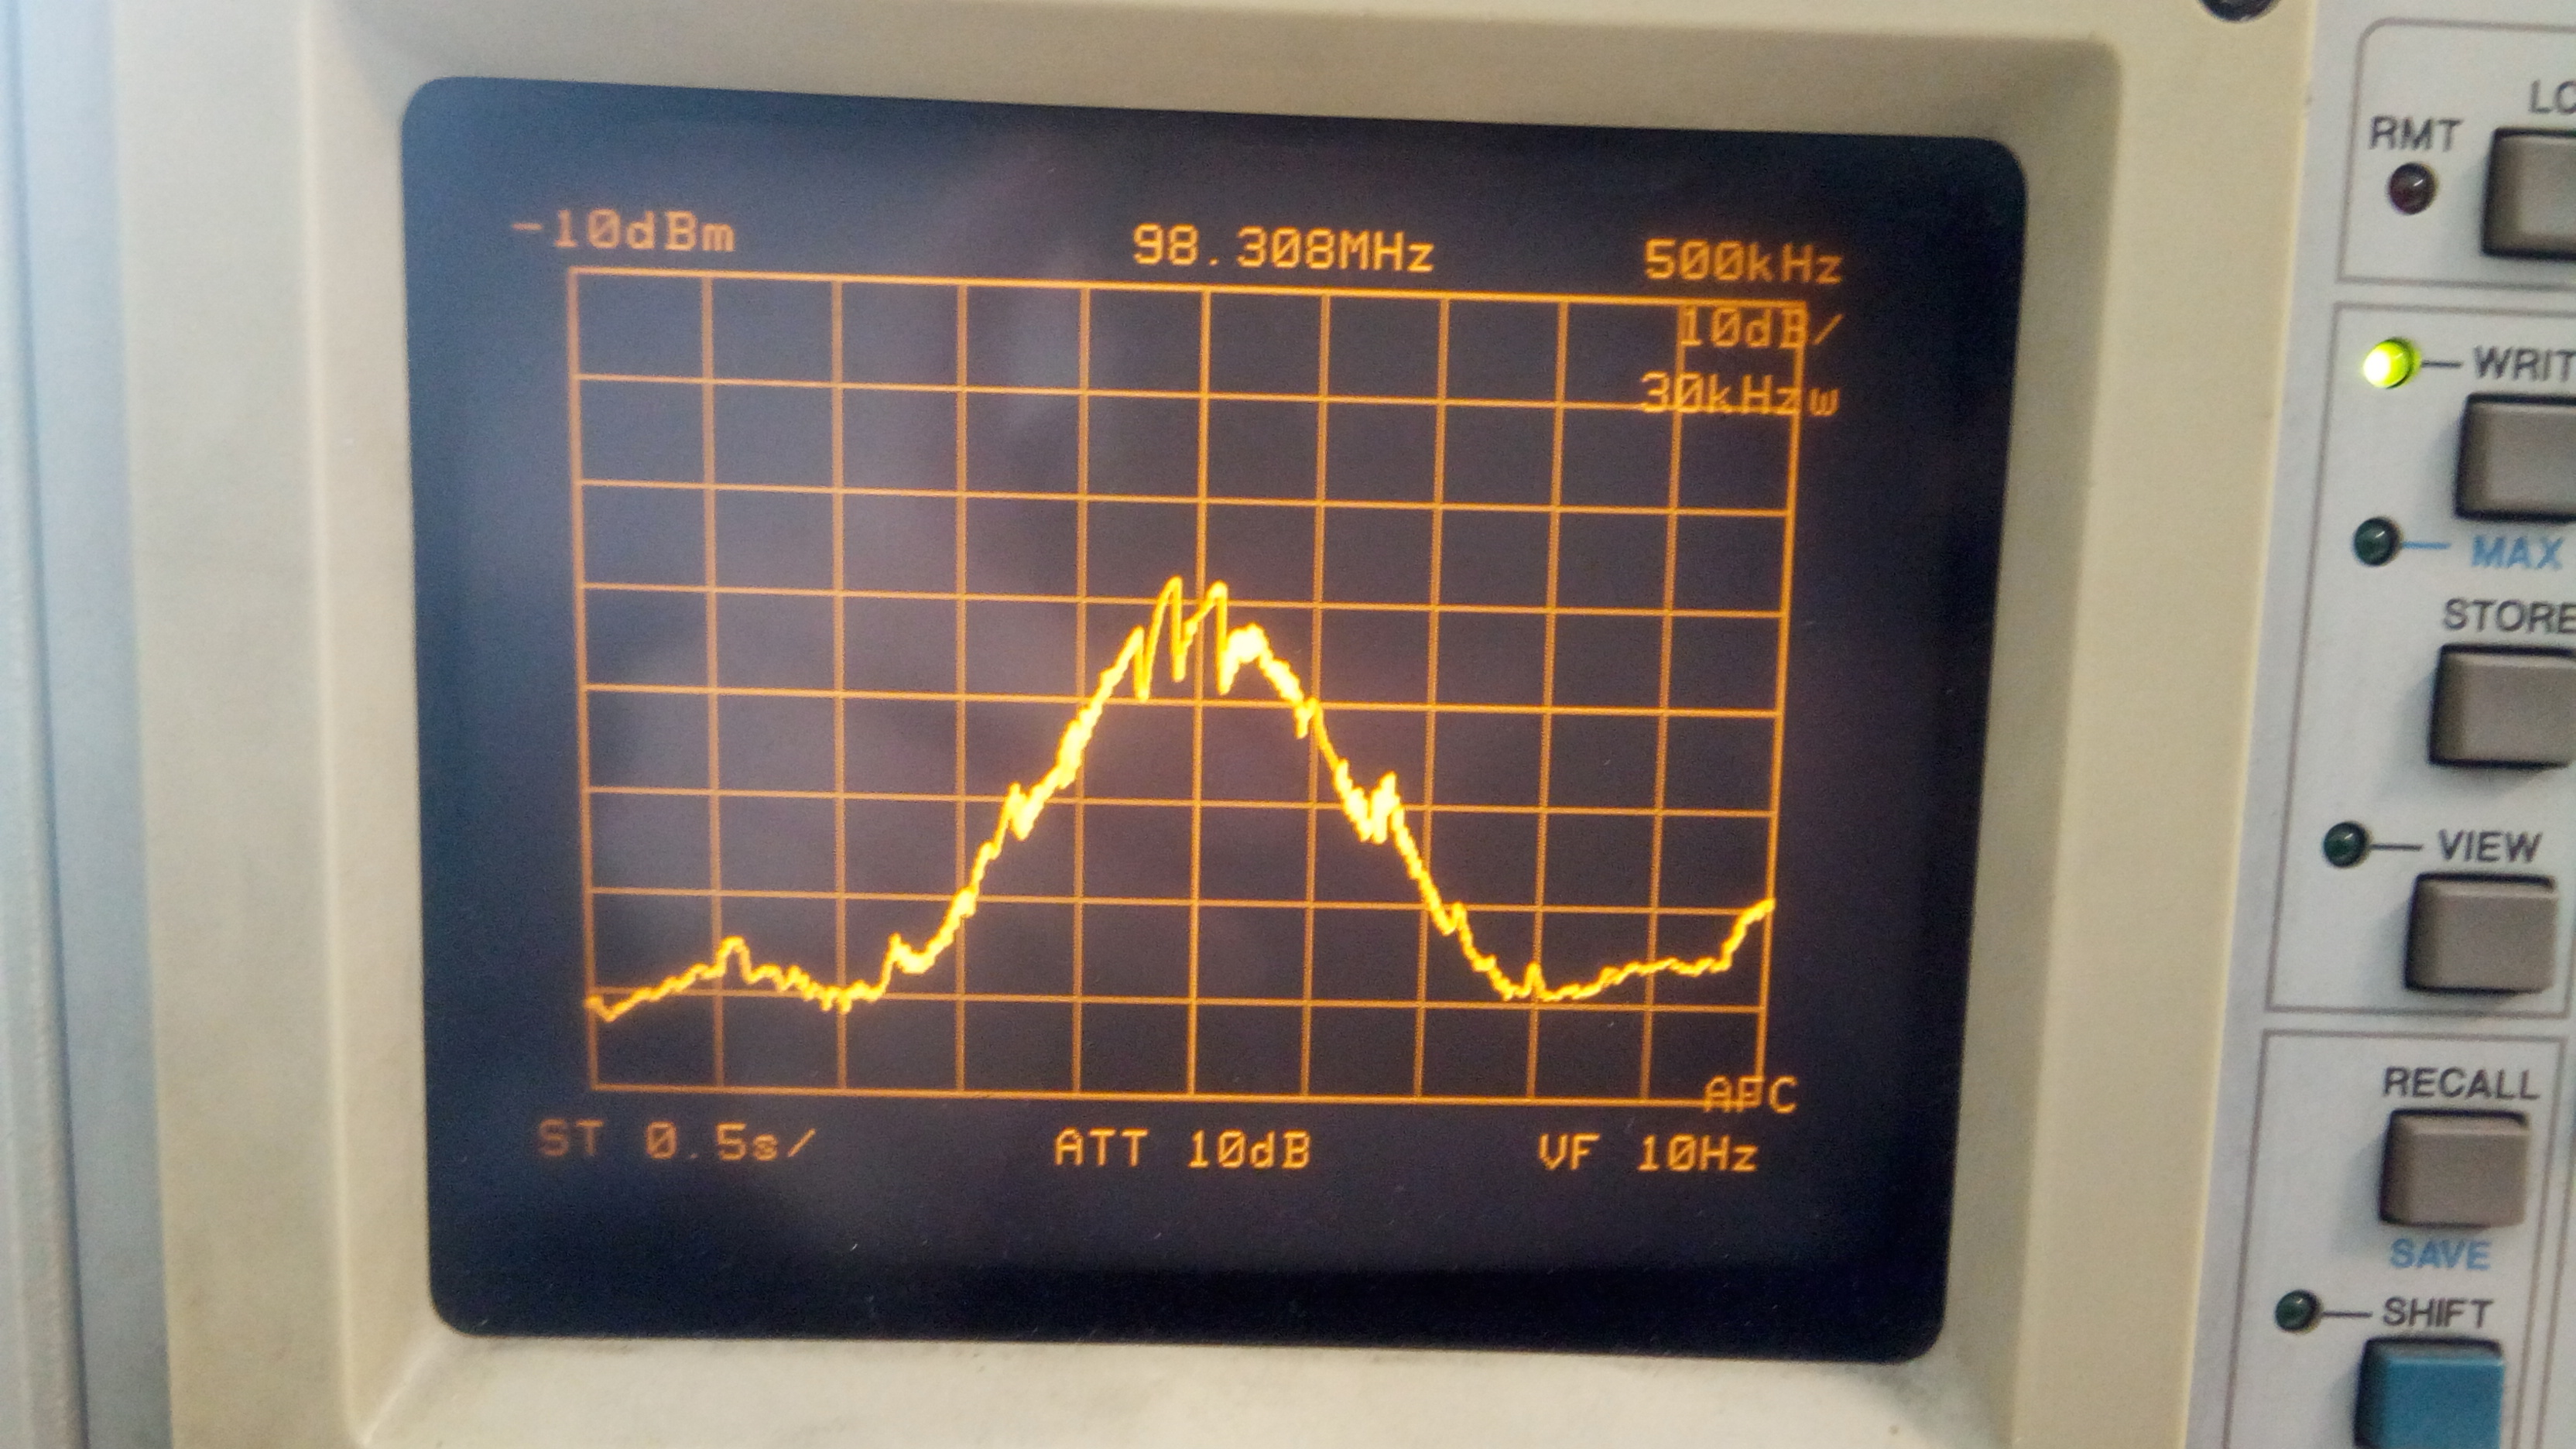
\includegraphics[width=0.9\textwidth]{/ImagenesEjercicio5-6y7/Mega9832.jpg}
\caption{Espectro medido para la emisora Mega 98.3}
	\label{fig:mega}
\end{figure}

\begin{figure}[H]
	\centering
	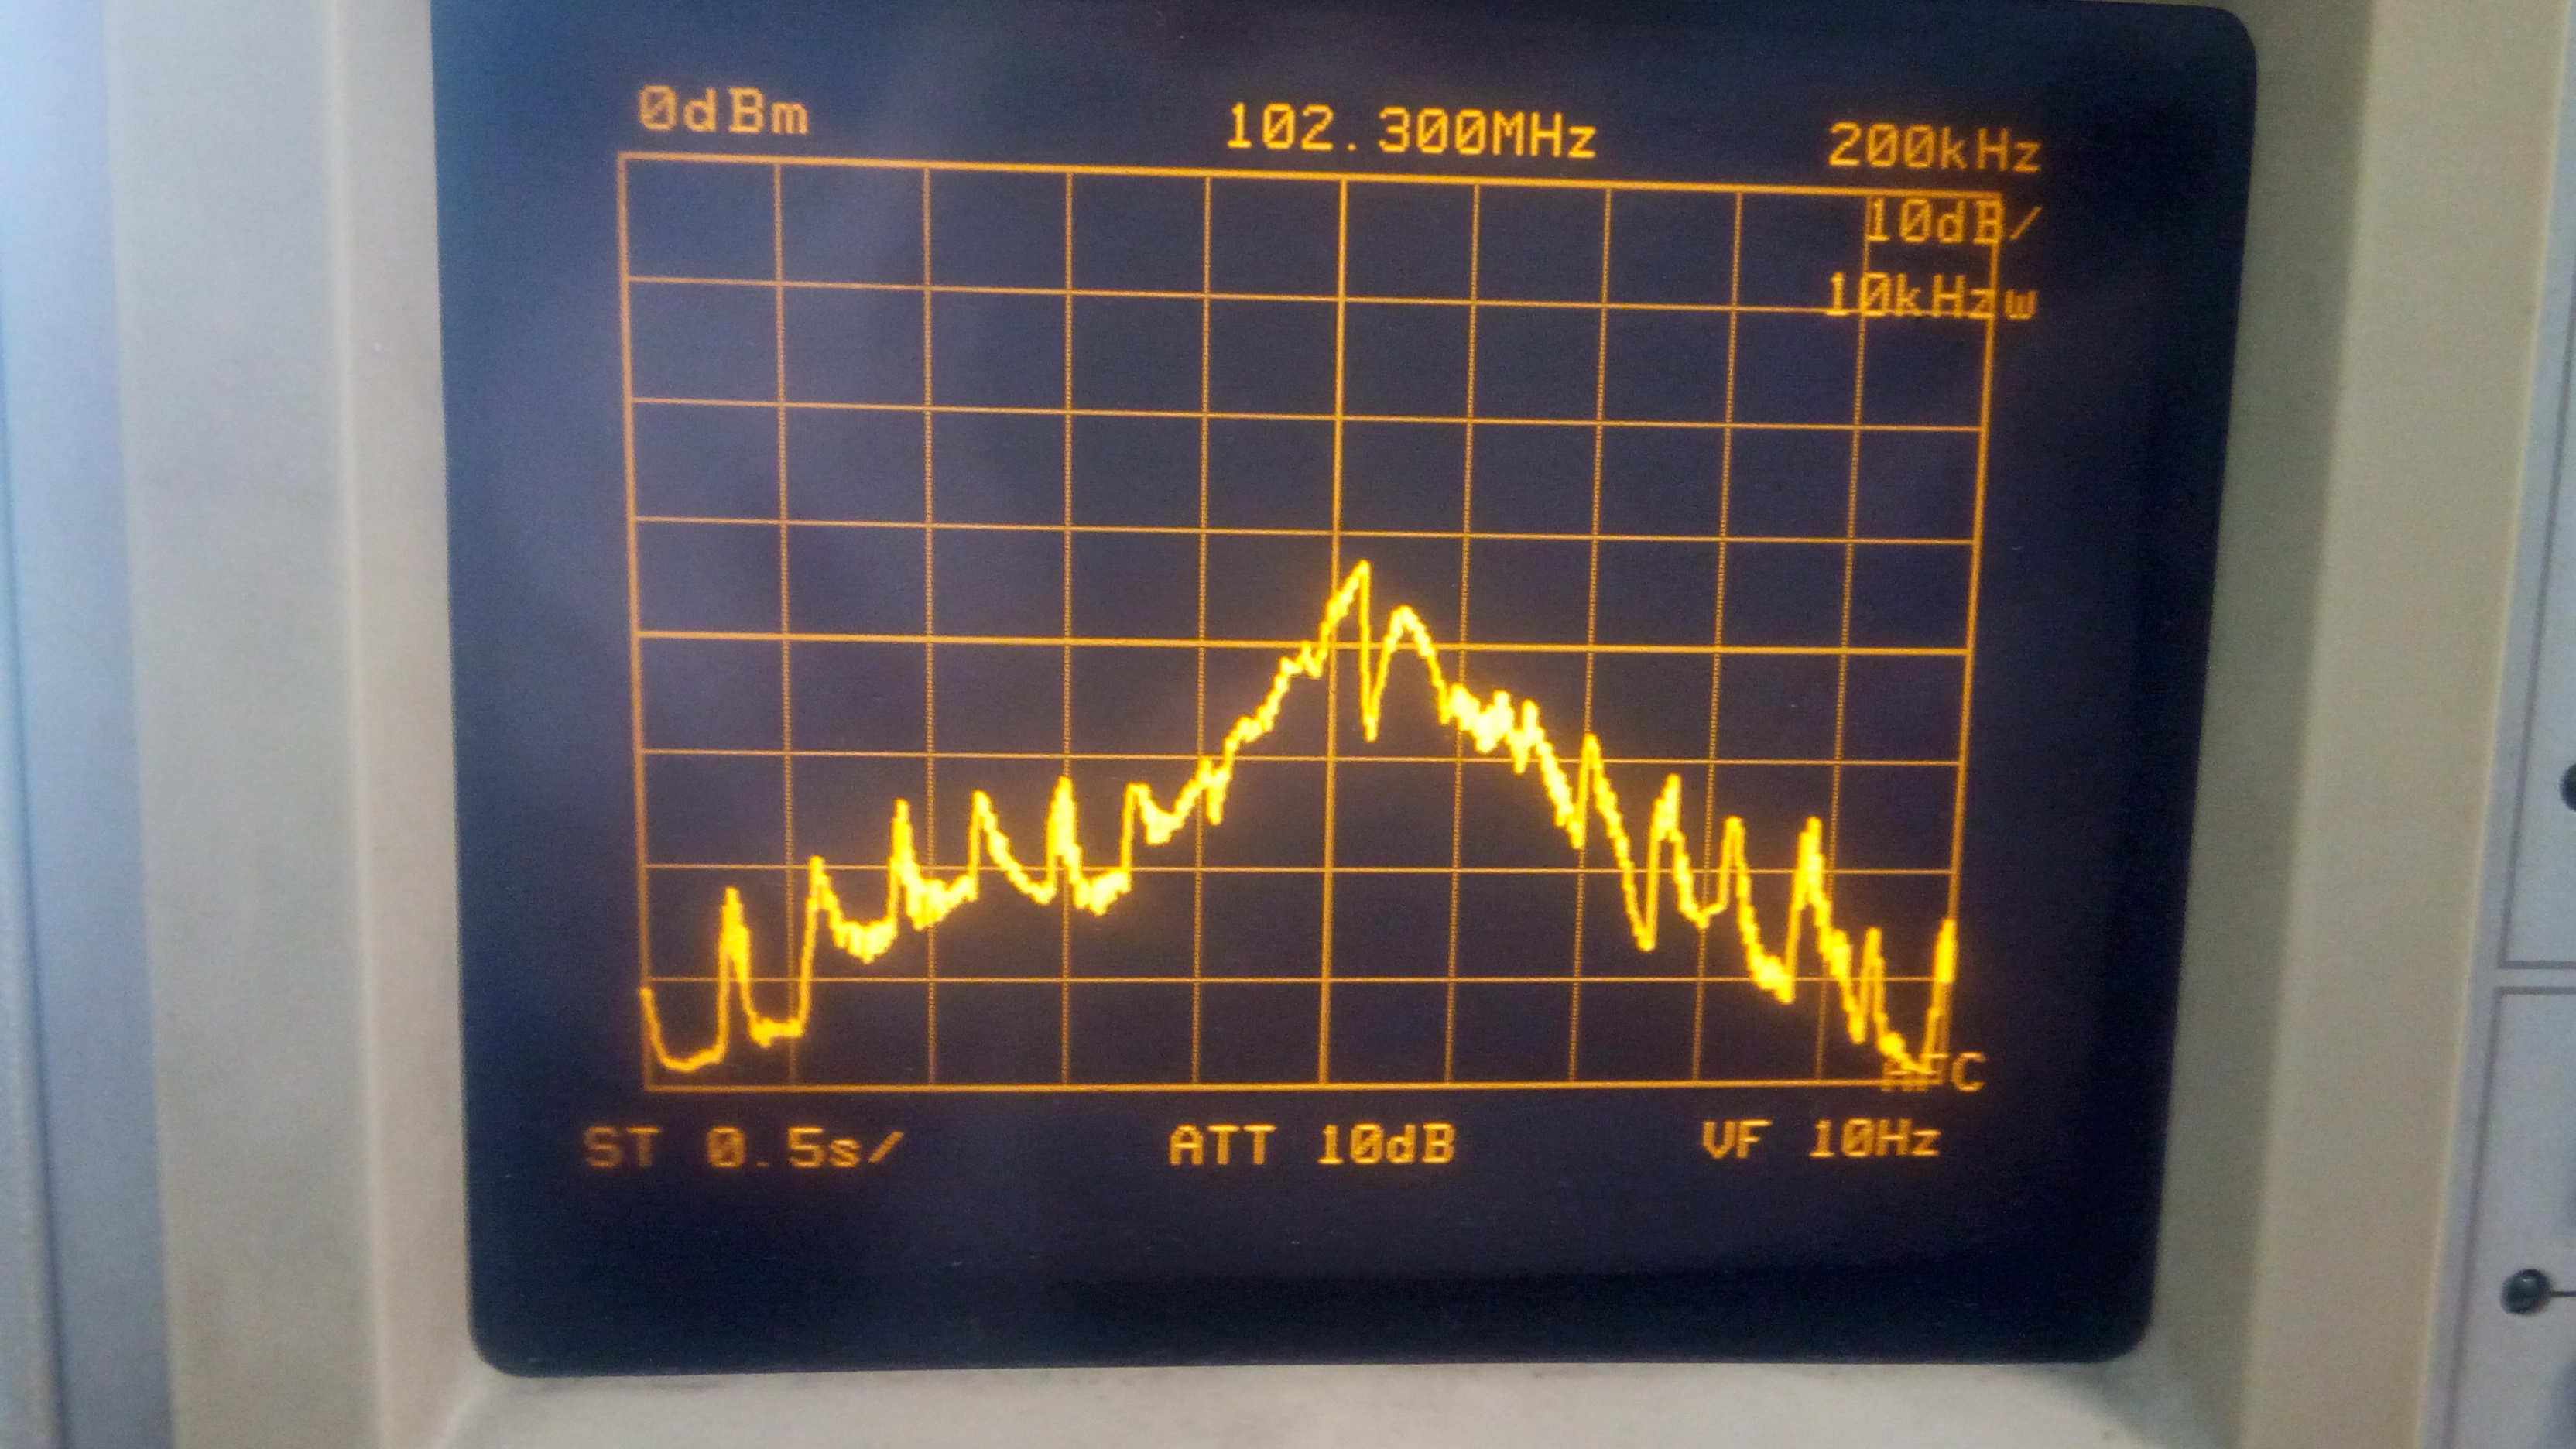
\includegraphics[width=0.9\textwidth]{/ImagenesEjercicio5-6y7/radioaspen1023.jpg}
\caption{Espectro medido para radio Aspen}
	\label{fig:aspen}
\end{figure}

\section{Señales de televisión}

De manera similar a lo que ocurre con las señales de FM, el espectro de frecuencias asignado a la televisión se encuentra dividido en bandas:
\begin{itemize}
    \item Banda I - VHF: de 54MHz a 88MHz 
    \item Banda II - VHF: de 174MHz a 216MHz 
    \item Banda III - UHF: de 512MHz a 806MHz
\end{itemize}

A su vez, el espectro está dividido en canales desde el 2 al 69. A cada canal le corresponden $6 MHz$. Los canales del 2 al 6 se encuentran en la banda I, los canales del 7 al 13 en la banda II y los canales del 21 al 69 (excluyendo al 37 que corresponde a radioastronomía) en la banda III.

Las bandas se puede dividir en distintas categorías según su radio de servicio. Dichas categorías para la banda II se presentan en la Figura (\ref{fig:ctt})

\begin{figure}[H]
	\centering
	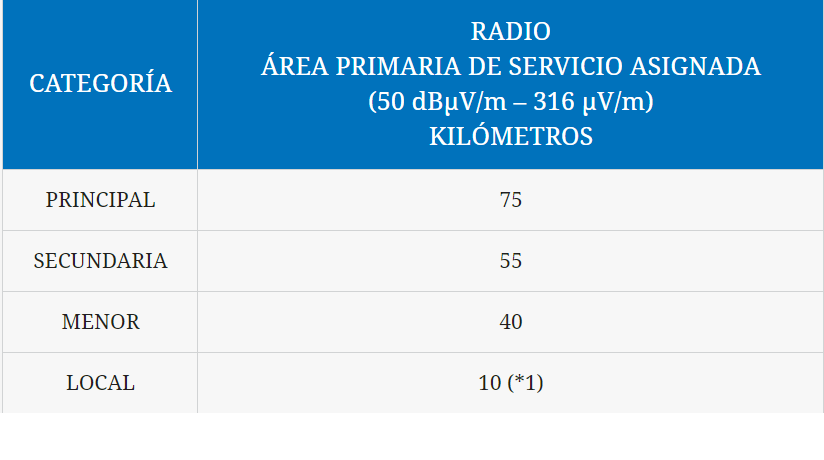
\includegraphics[width=0.6\textwidth]{/ImagenesEjercicio5-6y7/ctt.png}
	\caption{Categorías para Canal II}	
	\label{fig:ctt}
\end{figure}

El Canal 11 tiene asignada la banda de frecuencia de 198 MHz a 204 MHz. Se logró sintonizar la portadora de audio y se esuchó con los parlantes el programa siendo emitido en ese momento. En la Figura (\ref{fig:canal11}) se presenta lo observado en el analizador al sintonizar la portadora. En la Tabla 
(\ref{tab:ch}) se muestra cómo están distribuidas las portadores de video y audio para este canal.

\begin{table}[H]
\centering
\begin{tabular}{|l|l|}
\hline
Frecuencia & Contenido             \\ \hline
199,25     & Portadora de video    \\ \hline
202,83     & Subportadora de color \\ \hline
203,85     & Portadora de sonido   \\ \hline
\end{tabular}
\caption{Frecuencias para Canal 11}
\label{tab:ch}
\end{table}

\begin{figure}[H]
	\centering
	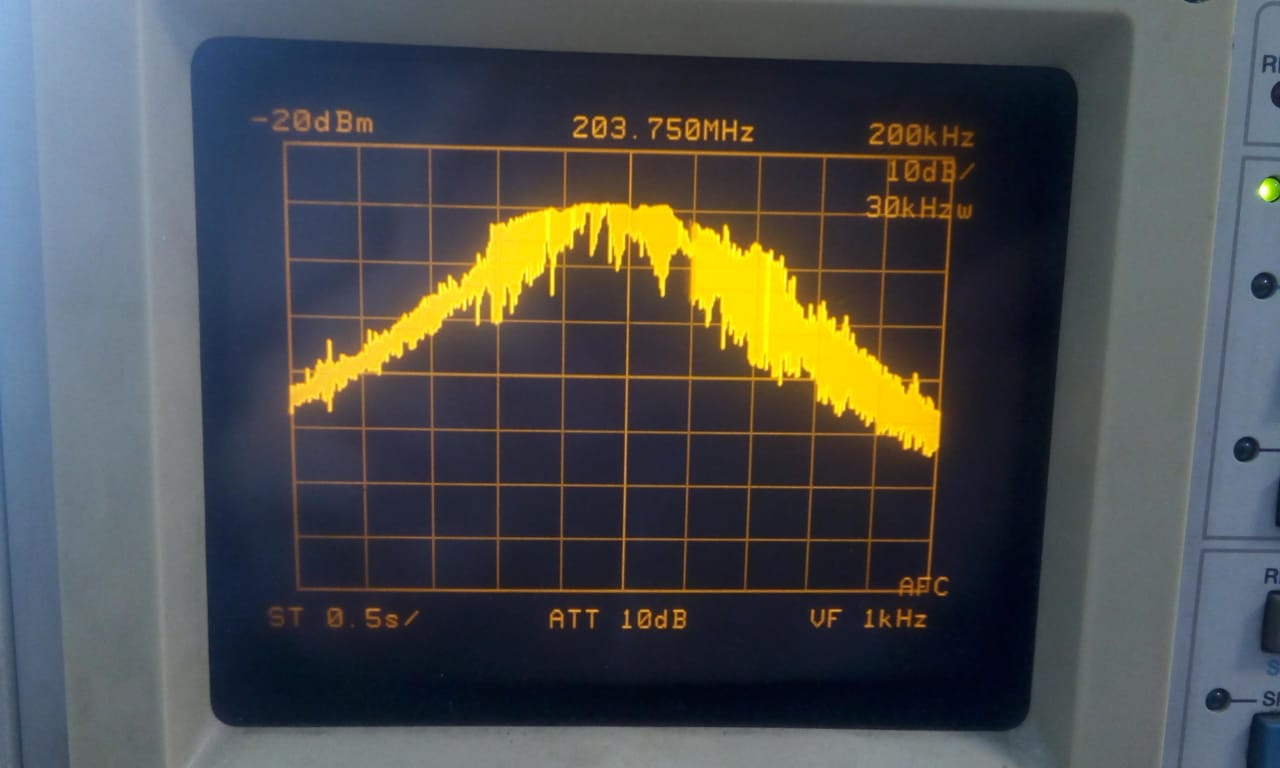
\includegraphics[width=0.9\textwidth]{/ImagenesEjercicio5-6y7/canal11_2.jpeg}
	\caption{Espectro de audio de canal 11}	
	\label{fig:canal11}
\end{figure}

